\documentclass{instructions}

\usepackage{alltt}
\usepackage{xspace}

\newcommand{\git}{\texttt{git}\xspace}
\newcommand\bs{\char`\\}

\graphicspath{{figs/}}

\title{A Robotic Arm from Scratch}
\subtitle{}
\date{\today}

\illustration{proj1}

\summary{

This project is about \textbf{designing your own robotic arm} (with at least 2
degrees of freedom, but you can add more), \textbf{programming it with ROS},
building a
\textbf{3D visualisation} for it, and, if time permit, using a \textbf{3D motion
planner} to control it automatically!

Be ready to \textbf{design \& 3D print} the parts of your robot, \textbf{program
an Arduino to control servo-motors} and \textbf{solder bits together}!

}

\objectives{}

\challenges{}

\begin{document}

\maketitle

%
%\note{
%    As usual, \textbf{document in your lab journal your findings}.
%Add \textbf{code snippets}, \textbf{screenshots}, \textbf{pictures} and link to \textbf{videos} as needed.
%
%\vspace{1em}
%
%And do not forget: \textbf{write your lab journal as a text file using the Markdown
%syntax} and \textbf{push your journal and the pictures on GitHub}.
%
%}

%%%%%%%%%%%%%%%%%%%%%%%%%%%%%%%%%%%%%%%%%%%%%%%%%%%%%%%%%%%%%%%%%%
%%%%%%%%%%%%%%%%%%%%%%%%%%%%%%%%%%%%%%%%%%%%%%%%%%%%%%%%%%%%%%%%%%
%%%%%%%%%%%%%%%%%%%%%%%%%%%%%%%%%%%%%%%%%%%%%%%%%%%%%%%%%%%%%%%%%%

\pagebreak

\part{Getting started with the Robotic Arm mini-project}

This project is about \textbf{designing your own robotic arm} (with at least 2
degrees of freedom, but you can add more), \textbf{programming it with ROS},
building a
\textbf{3D visualisation} for it, and, if time permit, using a \textbf{3D motion
planner} to control it automatically!

\begin{figure}[h!]
    \centering
    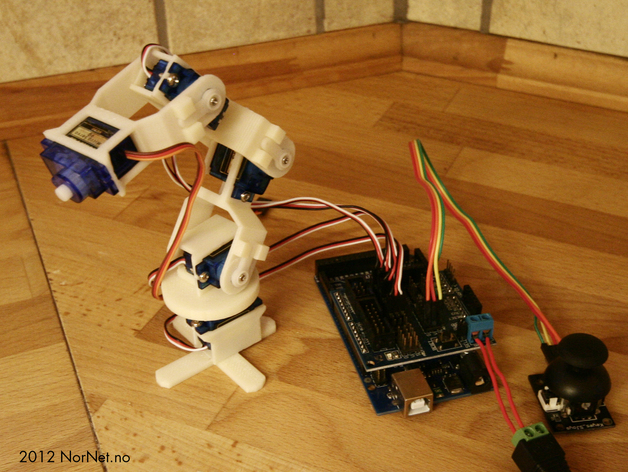
\includegraphics[width=0.32\linewidth]{servo-arm}
    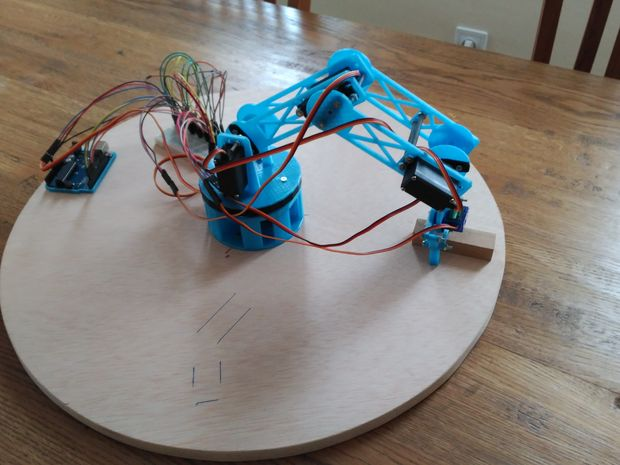
\includegraphics[width=0.32\linewidth]{servo-arm2}
    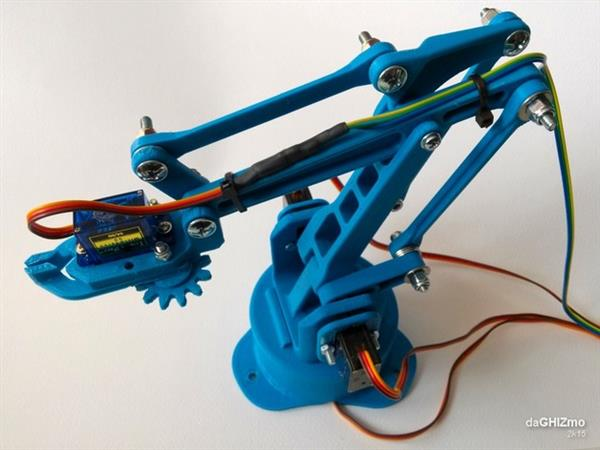
\includegraphics[width=0.32\linewidth]{servo-arm3}
    \caption{Three examples of 3D printed arms. The first one has 5 degrees of
    freedom, the second one 4 DoFs, the last one 3 DoFs.}
    \label{}
\end{figure}

\note{ For this project, it is best to \textbf{work in pairs}, but feel free to start
alone or to form a bigger group if you prefer.}

\vspace{2em}
\textbf{Indicative working plan}

\begin{itemize}
    \item \textbf{Week 1}:  control of two servo-motors with the Arduino; use of 
        potentiometers to control them
    \item \textbf{Week 2}: Mock-up arm with cardboard; refresher on 3D design
        with SolidWorks with Julian; start of the 3D printing
    \item \textbf{Week 3}: Design of the arm continued; arm assembly
    \item \textbf{Week 4}: ROS on Arduino; control of the servo using ROS
    \item \textbf{Week 5}: 3D model of the arm, visualisation of the arm in RViz
    \item \textbf{Week 6}: Finalisation of arms; if time permit, 3D motion
        planning using ROS
\end{itemize}

\begin{figure}
    \centering
    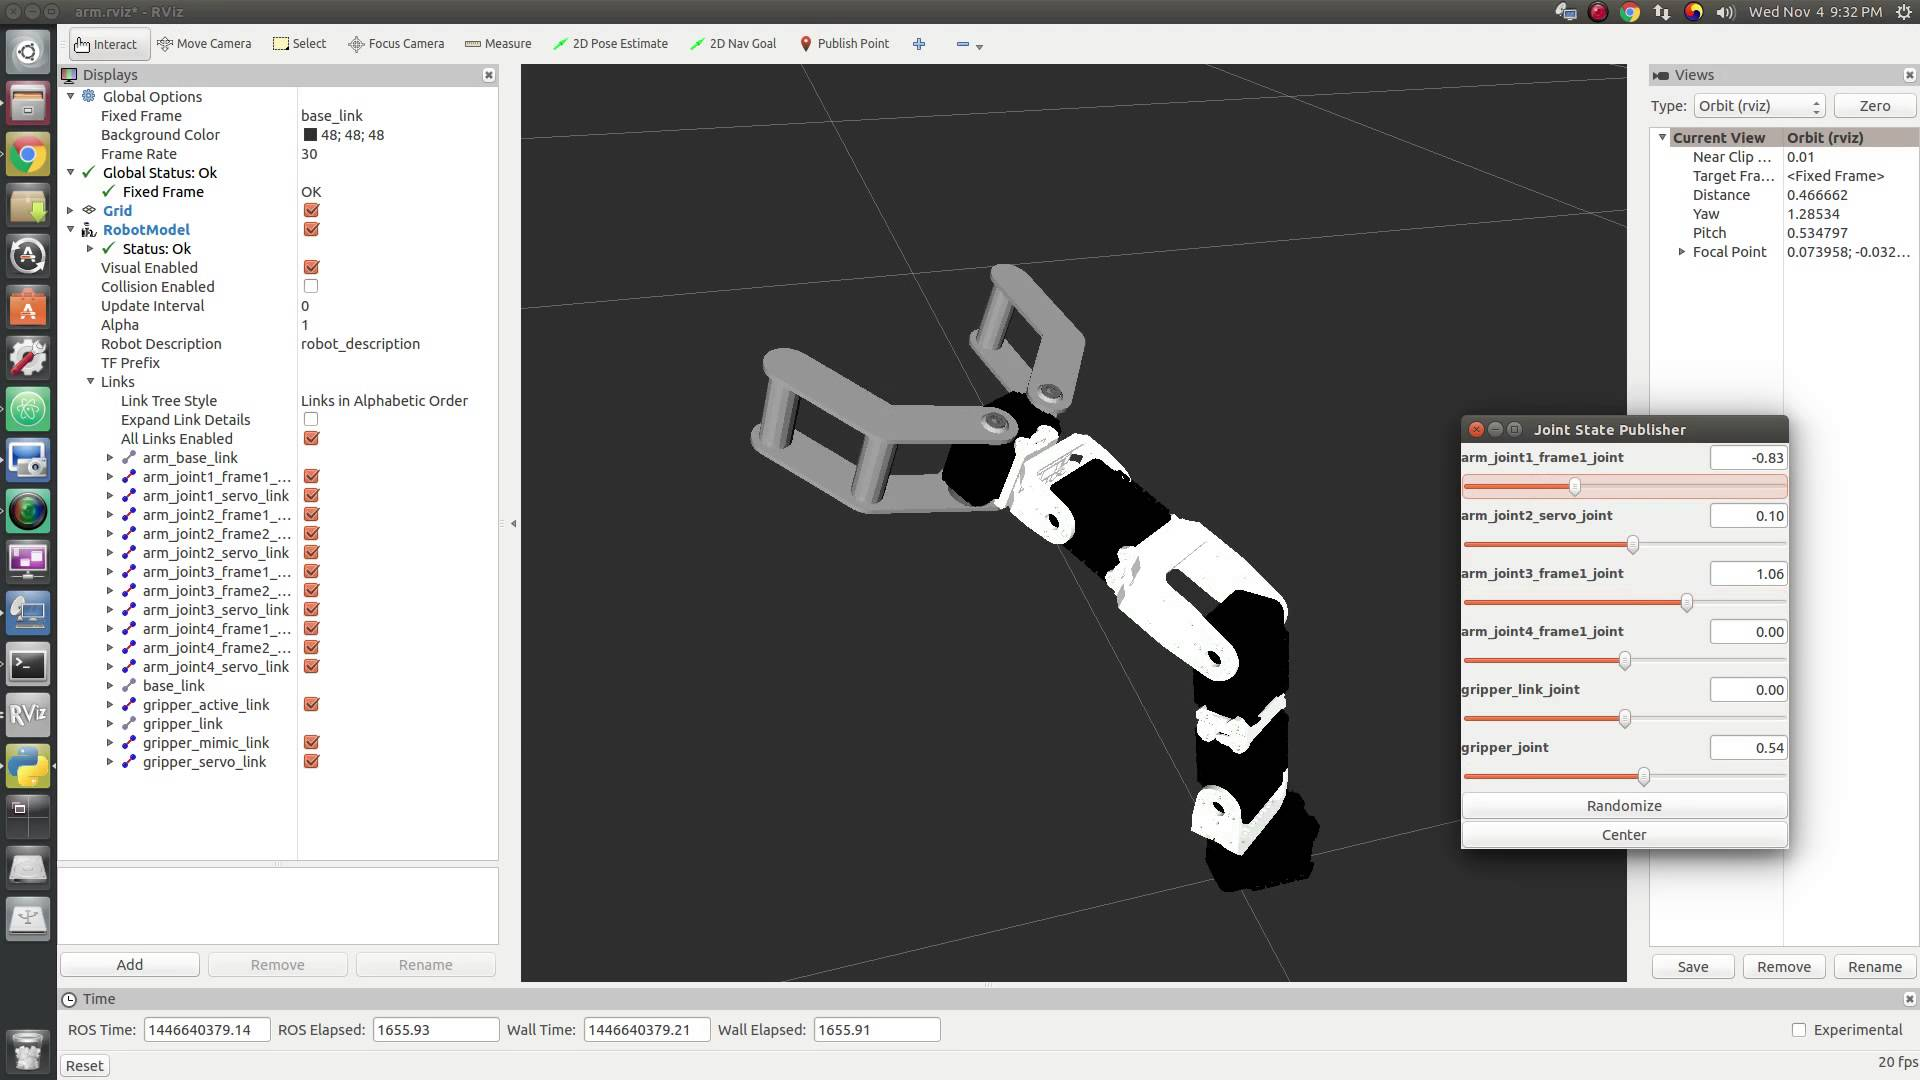
\includegraphics[width=0.9\linewidth]{servo-rviz}
    \caption{Later during the project, you will create a 3D interface to control
    your arm, using the standard ROS tools like RViz, pictured here.}
    \label{}
\end{figure}

\pagebreak

~

%%%%%%%%%%%%%%%%%%%%%%%%%%%%%%%%%%%%%%%%%%%%%%%%%%%%%%%%%%%%%%%%%%
%%%%%%%%%%%%%%%%%%%%%%%%%%%%%%%%%%%%%%%%%%%%%%%%%%%%%%%%%%%%%%%%%%
%%%%%%%%%%%%%%%%%%%%%%%%%%%%%%%%%%%%%%%%%%%%%%%%%%%%%%%%%%%%%%%%%%
\part{Servo-motor control with an Arduino}

\step{Get ready} First, get from the workshop 2 RC mini-servos as well as an Arduino board and
two potentiometers.

\note{Take a plastic bin as well, that you can label with you names. The bins
can be left in the lockers when you are not working on your project.}


\more{
    If you wish, you can create a design with additional degrees of freedom.
    You can borrow more servos from the workshop. You may as well want to source
    additional actuators by
    yourselves: small servo-motors or stepper motors can be found online for less than 5 pounds.
}

The RC servomotor (Fig. \ref{servo}) is a unit consisting of a small electric
motor driving a gear train. It often uses a potentiometer to measure
angular position measurement. Often such a unit is small and cheap
although more expensive designs using metal gears and digital control
circuitry are also available.

\begin{figure}[h!]
    \centering
    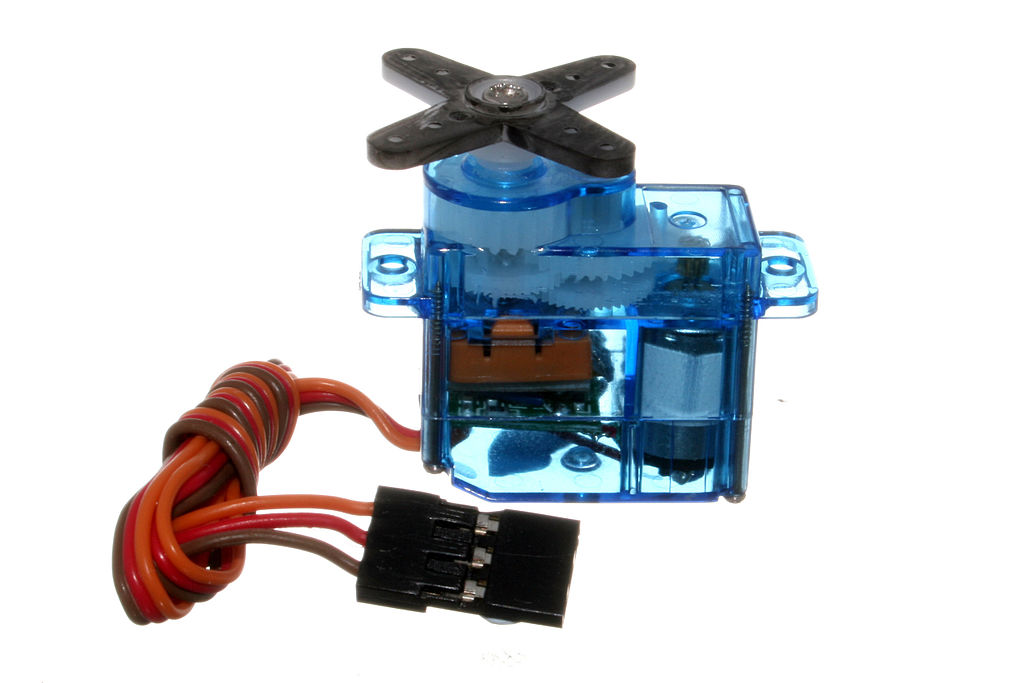
\includegraphics[width=0.6\linewidth]{figs/servo1}
    \caption{Micro servo motor}
    \label{servo}
\end{figure}


The RC servo generally incorporates circuitry that implements position
feedback control (Fig. \ref{closedloop}). The output position is compared to the commanded
target position. This gives rise to an error signal. The error drives the
electric motor in appropriate direction. When it becomes zero the servo
stops moving and reaches equilibrium. A position servomotor usually
sets the output target angle through the width of a control signal (pulse width) as show in
Fig.~\ref{pwm}.

\begin{figure}[h!]
    \centering
    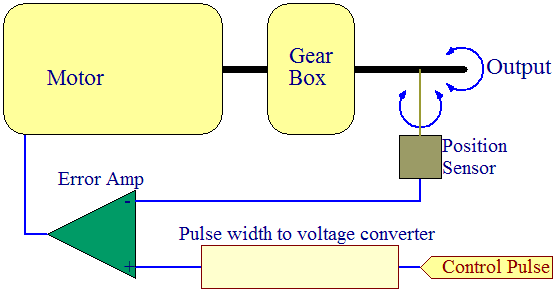
\includegraphics[width=0.6\linewidth]{figs/servo2}
    \caption{RC servo control showing feedback pathways}
    \label{closedloop}
\end{figure}

A RC servomotor typically has three connections:

\begin{itemize}
    \item The black wire is usually the ground, the red wire is connected to
        $V_{ref}$ (5V)
    and the white (or yellow) wire is the control pulse input.
\item If this is not the case on your servo, check its datasheet
\item You will need pins to connect the female plug to the female Arduino
  outputs
\end{itemize}

\begin{figure}[bh!]
    \centering
    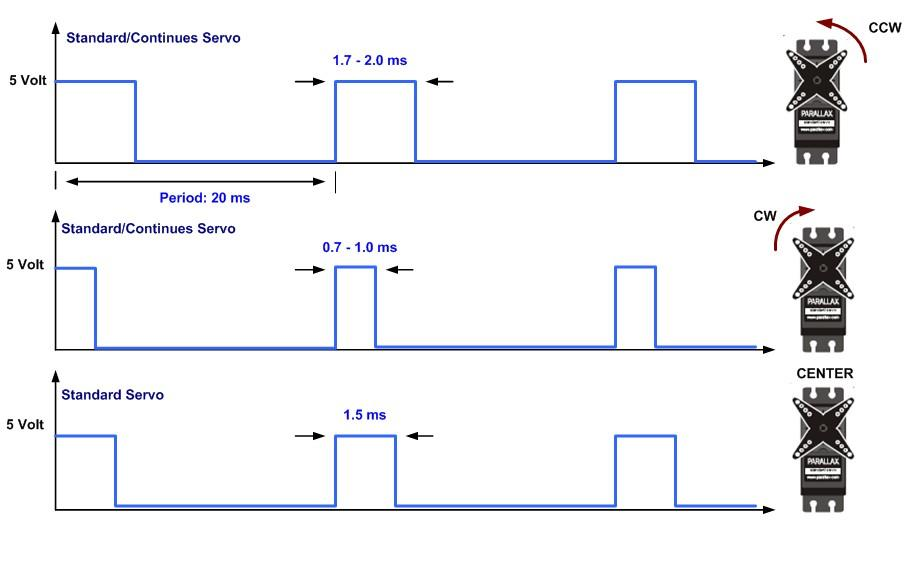
\includegraphics[width=0.7\linewidth]{figs/servo-pwm}
    \caption{RC servo operation by pulse width control}
    \label{pwm}
\end{figure}

\step{Control an RC servo}

\begin{center}
    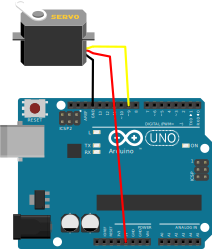
\includegraphics[width=0.4\linewidth]{servo-arduino}
\end{center}

\begin{enumerate}
\item Attach the RC servo power connections to the Arduino power output pins
\item Attach the control input to a PWM output pin on the Arduino (\eg
  port 9)
\item Write a simple program that runs the servo to generate an output
  movement back and forward over its entire range so its movement
  follows a low frequency sine wave of frequency around 0.2Hz. Use the code
        below as a starting point.

\end{enumerate}

\begin{cppcode}

#include <Servo.h>

Servo myservo;  // create servo object

int val;    // variable to read analog value

void setup() {
  myservo.attach(9);  // attaches the servo on pin 9
}

void loop() {
  val = 10;
  myservo.write(val); // sets the servo position
  delay(15); // waits for the servo to get there
}

\end{cppcode}

\step{Control the servo with a potentiometer}

\begin{center}
    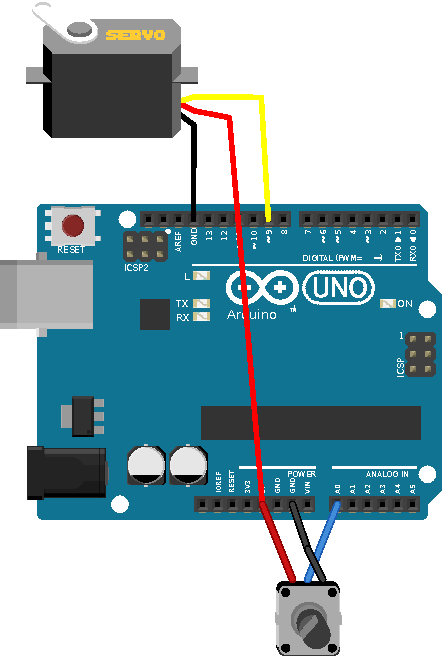
\includegraphics[width=0.4\linewidth]{servo-potentiometre-arduino}\hspace{2em}
    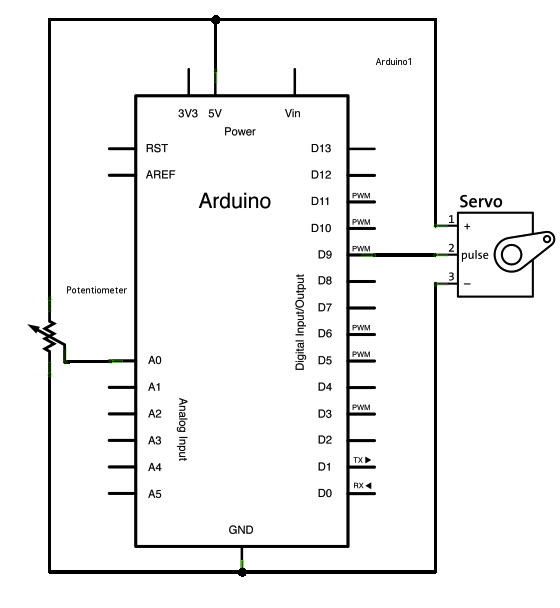
\includegraphics[width=0.4\linewidth]{knob_schem}
\end{center}

\begin{enumerate}
    \item Wire the provided potentiometer to one of the Arduino analog port.
        Write a program that reads the value of the potentiometer and writes it
        onto the serial port.
    \item Use the potentiometer to rotate the servo-motor.
\end{enumerate}

The code below reads the potentiometer. Look online for way to display back this
value using the \cpp{SerialPort}.

\begin{cppcode}

int potpin = 0;  // analog pin used for potentiometer
int val;    // variable to read analog value

void loop() {
  val = analogRead(potpin); // reads potentiometer
  val = map(val, 0, 1023, 0, 180); // remap values from 0 - 1023 to 0 - 180
}

\end{cppcode}


\step{A robot arm mock-up}

\begin{enumerate}
    \item Using pieces of cardboard, create an arm and attach it to the motor
        shaft (you can draw inspiration from the picture below, or come up with
        your own ideas)
    \item Estimate the torque of the servo-motor by hanging a fixed mass to the
        arm, at increasing distance of the motor shaft. Document the process,
        and check your estimate using the servo-motor datasheet (you can find it
        easily online)
    \item Modify your arm to insert the second servo motor
    \item Write a program that control both servos with the two provided
        potentiometers.
\end{enumerate}

\begin{figure}[h!]
    \centering
    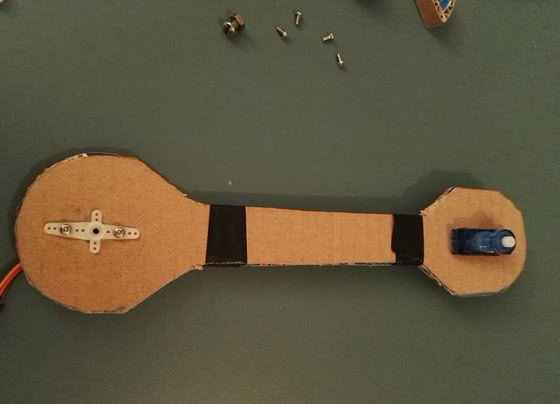
\includegraphics[width=0.9\linewidth]{figs/arm-cardboard}
    \caption{A possible assembly of 2 servos onto a cardboard arm. Taken from
    \url{http://www.instructables.com/id/CARDBIRD-the-Cardboard-Robotic-Arm/}}
    \label{}
\end{figure}


\part{Design and 3D print your arm}

Using the cardboard mock-up as an initial reference, design your arm in
SolidWorks.

Examples of designs from the previous years:

\begin{figure}[h!]
    \centering
    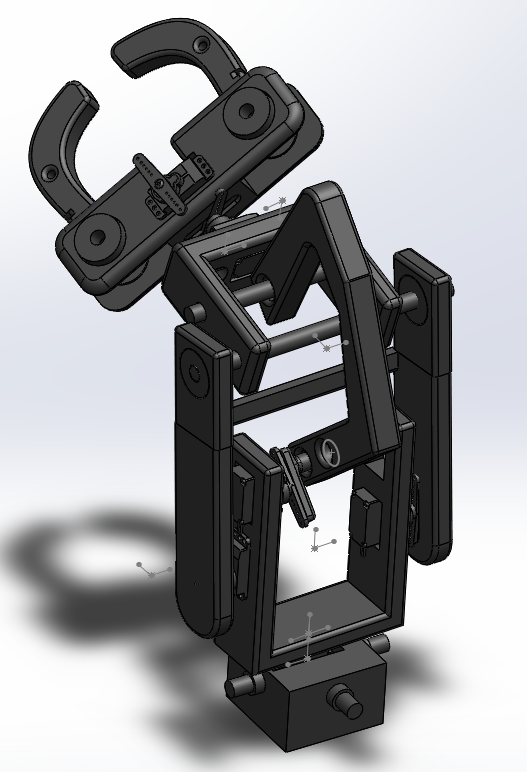
\includegraphics[height=6cm]{design3}
    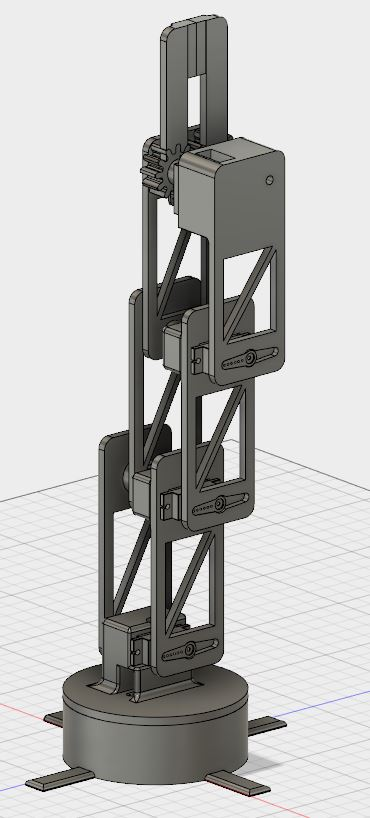
\includegraphics[height=6cm]{design1}
    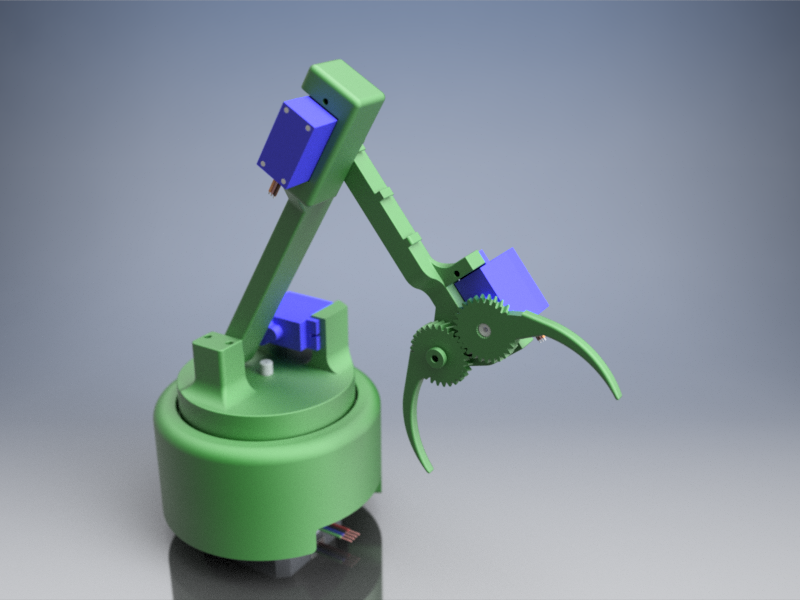
\includegraphics[height=6cm]{design2}
\end{figure}




\part{Servos control with ROS}

\step{Reboot on Linux}
    
Make sure you are running Linux. Otherwise, reboot and switch to Linux.
\textbf{ROS does not work on Windows}.

\step{Prepare the hardware}

Plug a servo to the Arduino, make sure you can get the servo to move using the
Arduino IDE and the following simple code sample:

\begin{cppcode}
#include <Servo.h>

Servo myservo;

int pos = 0;

void setup() {
  myservo.attach(9);  // attaches the servo on pin 9 to the servo object
}

void loop() {
  for (pos = 0; pos <= 180; pos += 1) {
    // in steps of 1 degree
    myservo.write(pos);
    delay(15);
  }
  for (pos = 180; pos >= 0; pos -= 1) {
    myservo.write(pos);
    delay(15);
  }
}
\end{cppcode}

\step{First steps with ROS}

You always need to start \sh{roscore} before being able to launch any other node.

Open a terminal and start it with the command \sh{roscore}.

In another window, type \sh{rostopic list} to list all the available topics. At
this point, you should only see two of them. Search on the web what is the use
of the \sh{/rosout} topic.

Let's publish something on a new topic. Type: 

\begin{shcode}
> rostopic pub /test std_msgs/String "Hello"
\end{shcode}

Now type again \sh{rostopic list}. You should see a new topic \sh{/test}.

Open a different terminal, and type \sh{rostopic echo /test} to display on the
console the messages exchanged on the \sh{/test} topic. Nothing should be
display at this point, since our \sh{"Hello"} message was published
\emph{before} we started \sh{rostopic echo}.

Try to publish another message on the \sh{/test} topic. This time, you should
see it.

\note{Quickly enough, you will end up with many terminal windows open at the
same time. You might find it usefule to use \texttt{ctrl+shift+t} to instead
create tabs in the same terminal window.}

As you have noticed, the \emph{type} of our \sh{/test} topic is
\sh{std_msgs/String}. ROS offers many standard datatypes. Start to familiarize
yourself with the basic message types by visiting
\href{http://wiki.ros.org/std_msgs}{wiki.ros.org/std\_msgs}.

\step{RViz}

RViz is the main 3D visualisation tool provided with ROS. Start it now (simply
type \sh{rviz} in a different terminal). At this point, RViz does not have much to
show (no ROS node is running yet, except... RViz itself), so the 3D viewport is
simply an empty grid (Figure~\ref{rviz}).

\begin{figure}[h!]
    \centering
    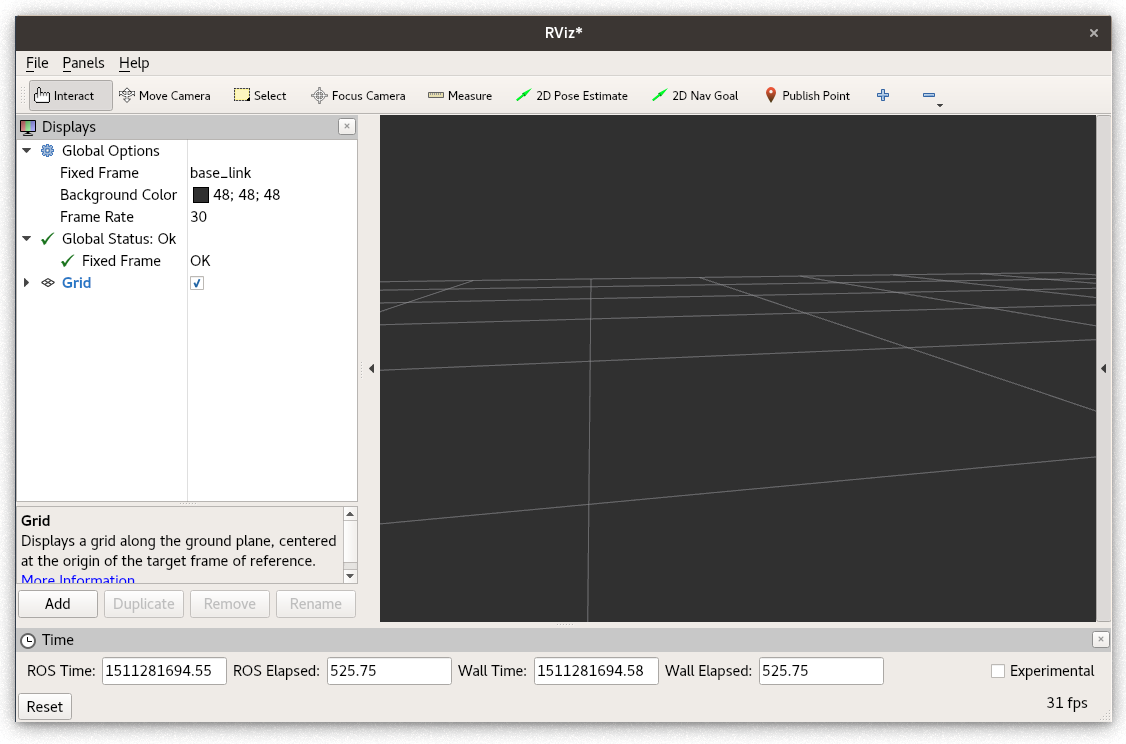
\includegraphics[width=0.7\linewidth]{rviz}
    \caption{The default, initial RViz window.}
    \label{rviz}
\end{figure}

RViz visualization rely on plugins: one plugin for every datatype we want to
visualise (images, 3D models, point clouds, etc.). Figure out how to add
visualisation plugins, and explore what is available.

\step{Configure ROS for the Arduino}

As the Arduino does not feature a network socket, we need to use a serial bridge
instead.  \sh{rosserial} is such a ROS \emph{bridge} that transparently
transport ROS messages over a serial connection.

\sh{rosserial_arduino} is a \sh{rosserial} \emph{client} for the Arduino (\ie
the library that runs \emph{on the Arduino} to deserialize the ROS messages).

It should alrady be installed on the computer. However, if this is not the case,
you can install \sh{rosserial} easily:

\begin{shcode}
> sudo apt install ros-melodic-rosserial-python ros-melodic-rosserial-arduino
\end{shcode}

To make it transparently available in the Arduino IDE, you also need to install
it as an Arduino library:

\begin{shcode}
> cd $HOME/sketchbook/libraries
> rosrun rosserial_arduino make_libraries.py .
\end{shcode}

Restart the Arduino IDE. You should now have access to many ROS examples
(Figure~\ref{ros-arduino-examples}).

\begin{figure}[h!]
    \centering
    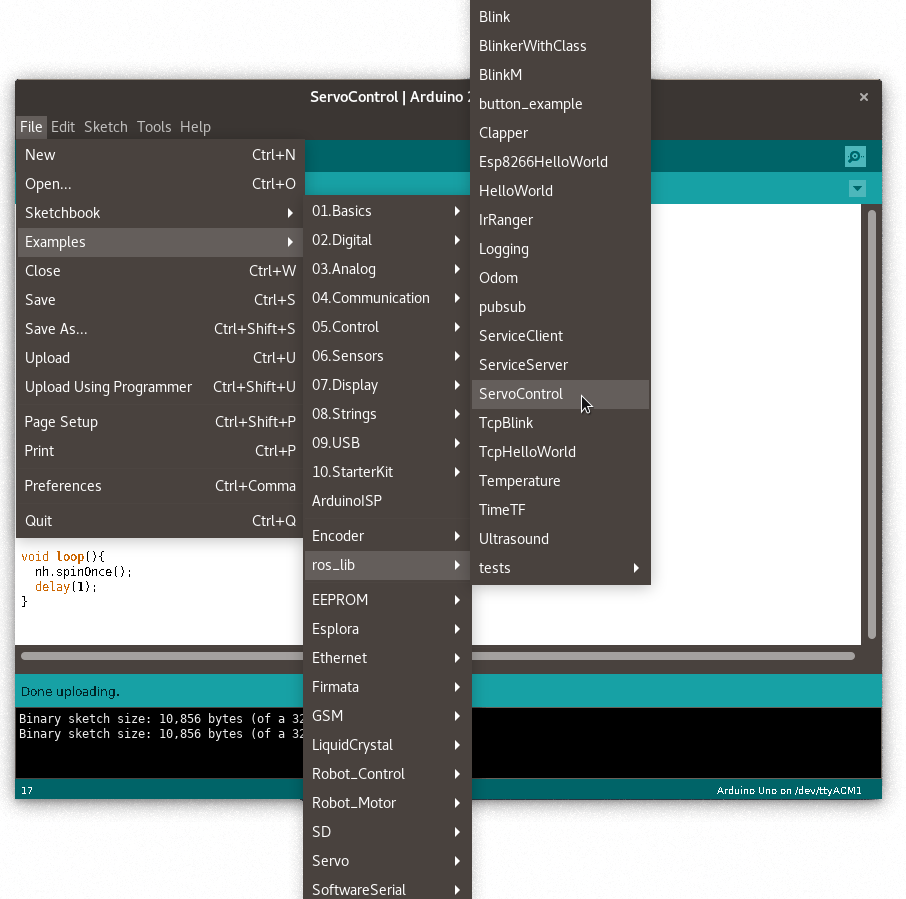
\includegraphics[width=0.56\linewidth]{arduino-ide-ros}
    \caption{Examples of ROS nodes for the Arduino}
    \label{ros-arduino-examples}
\end{figure}


\step{Write a ROS node for your Arduino}


Use the following code sample to control a servo by sending one integer between
0 and 180:

\begin{minted}[frame=lines,linenos=true]{cpp}
#include <ros.h>
#include <std_msgs/UInt16.h>
#include <Servo.h> 

using namespace ros;

NodeHandle  nh;
Servo servo;

void cb( const std_msgs::UInt16& msg){
  servo.write(msg.data); // 0-180
}

Subscriber<std_msgs::UInt16> sub("servo", cb);

void setup(){
  nh.initNode();
  nh.subscribe(sub);

  servo.attach(9); //attach it to pin 9
}

void loop(){
  nh.spinOnce();
  delay(1);
}

\end{minted}

\note{
    Analyse this code example. In particular, what is
the function defined at line 10, and the role of the object instantiated at line
14.
}

Compile and upload the code to the Arduino.

In a terminal, start \sh{rosserial} (changing the serial port of your Arduino as
required):

\begin{shcode}
> rosrun rosserial_python serial_node.py /dev/ttyACM0
\end{shcode}

Now, call \sh{rostopic pub} with the adequate parameter to move your servo-motor.

\part{3D model of your arm}

We have a first ROS node, able to control a servo motor. However, to do useful
things with our arm (like 3D motion planning), we need to describe its complete
kinematic model.

The next step is indeed to build a 3D model of the arm. We need to create a
\textbf{geometric and kinematic description of the arm} using the \textbf{URDF
format}.

\step{Visualise an existing URDF file in RViz}

Create a new directory called \sh{robot-project} and a sub-directory called
\sh{models}. Save the following URDF file in this subdirectory as
\sh{robot-arm.urdf}.

\note{
    You can also
    \href{https://github.com/hacker-space-brl/robotic-arm/code}{download
    this file from the GitHub repo}.
}

\begin{xmlcode}
<?xml version="1.0"?>
<robot name="roco_arm">
  <link name="base_link">
    <visual>
      <geometry>
        <cylinder length="0.06" radius="0.1"/>
      </geometry>
    </visual>
  </link>

  <link name="first_segment">
    <visual>
      <geometry>
        <box size="0.6 0.05 0.1"/>
      </geometry>
      <origin rpy="0 0 0" xyz="-0.3 0 0" />
    </visual>
  </link>

  <joint name="base_to_first" type="revolute">
    <axis xyz="0 1 0" />
    <limit effort="1000" lower="0"
                    upper="3.14" velocity="0.5" />
    <parent link="base_link"/>
    <child link="first_segment"/>
    <origin xyz="0 0 0.03" />
  </joint>
</robot>
\end{xmlcode}

Load this file as the \emph{description} of your robot: 

\begin{shcode}
> rosparam set robot_description -t models/robot-arm.urdf
\end{shcode}

Next, launch the \sh{robot_state_publisher} and \sh{joint_state_publisher} nodes
in two terminals:

\begin{shcode}
> rosrun robot_state_publisher robot_state_publisher
\end{shcode}

\begin{shcode}
> rosrun joint_state_publisher joint_state_publisher _use_gui:=true
\end{shcode}


The \sh{robot_state_publisher} node reads the robot description, and broadcasts the 6D transformations (TF
frames) corresponding to each of the links described in the URDF file.

The \sh{joint_state_publisher} node reads as well the robot description and
creates a GUI with one slider per joint, making it easy to manipulate the
pose of our robot.

Finally, add the \texttt{Robot model} plugin to RViz and set the \texttt{Fixed
frame} to \sh{/base_link} (Figure~\ref{rviz-robot-model}).


\begin{figure}[h!]
    \centering
    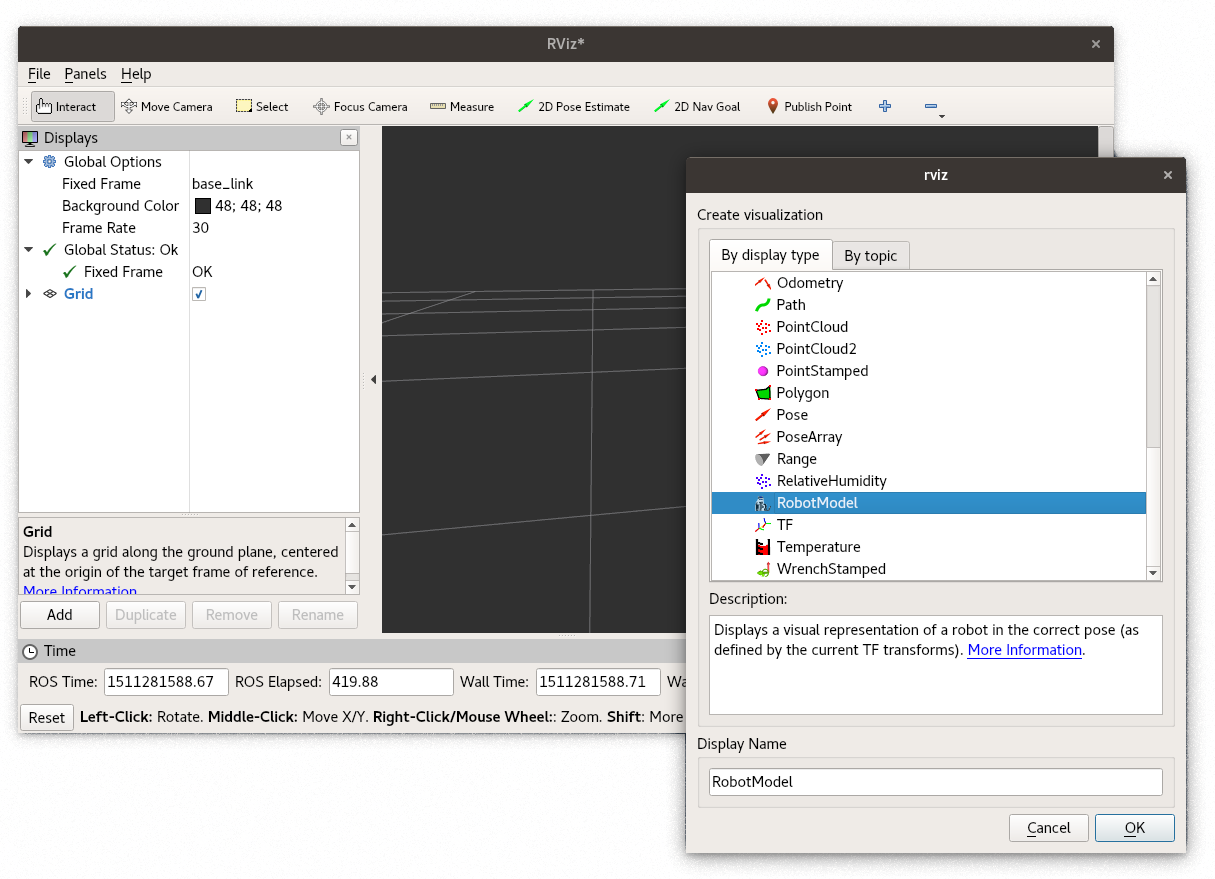
\includegraphics[width=0.52\linewidth]{rviz-plugins}
    \caption{Adding the \texttt{Robot model} visualisation plugin to RViz}
    \label{rviz-robot-model}
\end{figure}

\pagebreak
You should see the following model in the 3D viewport (Figure~\ref{rviz-urdf}):

\begin{figure}[h!]
    \centering
    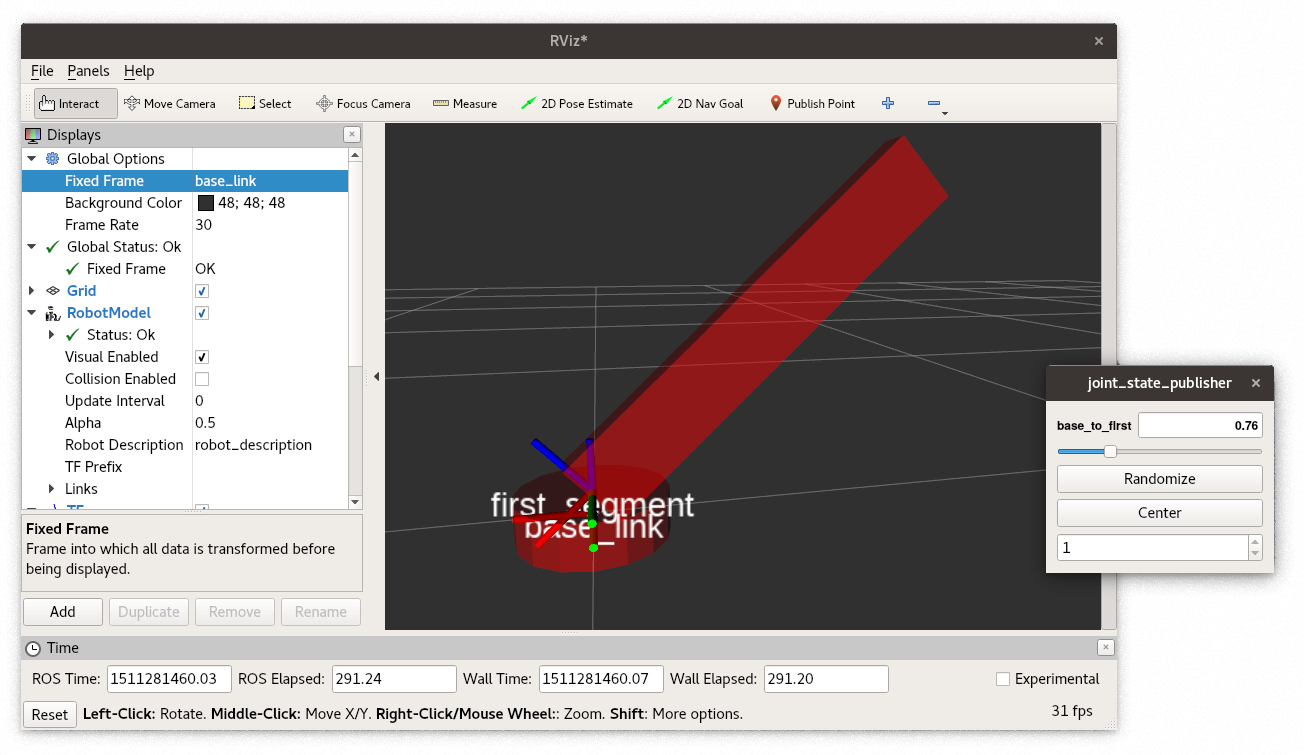
\includegraphics[width=0.9\linewidth]{urdf-rviz}
    \caption{A first, simple, URDF model, visualised in RViz. On the right, the
    \sh{joint_state_publisher} interface.}
    \label{rviz-urdf}
\end{figure}


\step{Create the URDF file of your robot}

Using \sh{robot-arm.urdf} as a starting point, complete the URDF to accurately
model your arm. Measure precisely the dimension of each segment, and position
accurately the joints.

\note{
You might find it useful to use your CAD software to quickly measure the
segments and the position of the joint axes.
}

\more{
    Some CAD tools (like Solidworks) have extensions to export directly to URDF.
    Check online!
}

If you wish to check your model, reload the robot description, and restart the
\sh{robot_state_publisher} and \sh{joint_state_publisher} nodes. You do not need
to restart RViz, but you need to desactivate and re-activate the \texttt{robot
model} plugin to update the rendering.

\more{
    Instead of simple geometric primitive, you can use STL meshes (like the ones
    you 3D printed) for the visuals of your arm. Check the
    \href{http://wiki.ros.org/urdf/XML/link}{URDF documentation} to learn how to
    do that.
}


\part{Control the servo-motors from the robot's joint state}

Lastly, modify the Arduino code to directly read the robot joint state and to
control the servo-motors accordingly.


\note{
    As short video-clip of your arm moving alongside the 3D model in RViz is
    certainly appropriate for your Twitter/Instagram account!
}


\part{Automatic motion planning}

The last step is to use ROS to plan a full arm motion. Check the
\href{https://ros-planning.github.io/moveit_tutorials/}{MoveIt! tutorials}, and
get your robot to move!

\begin{center}
    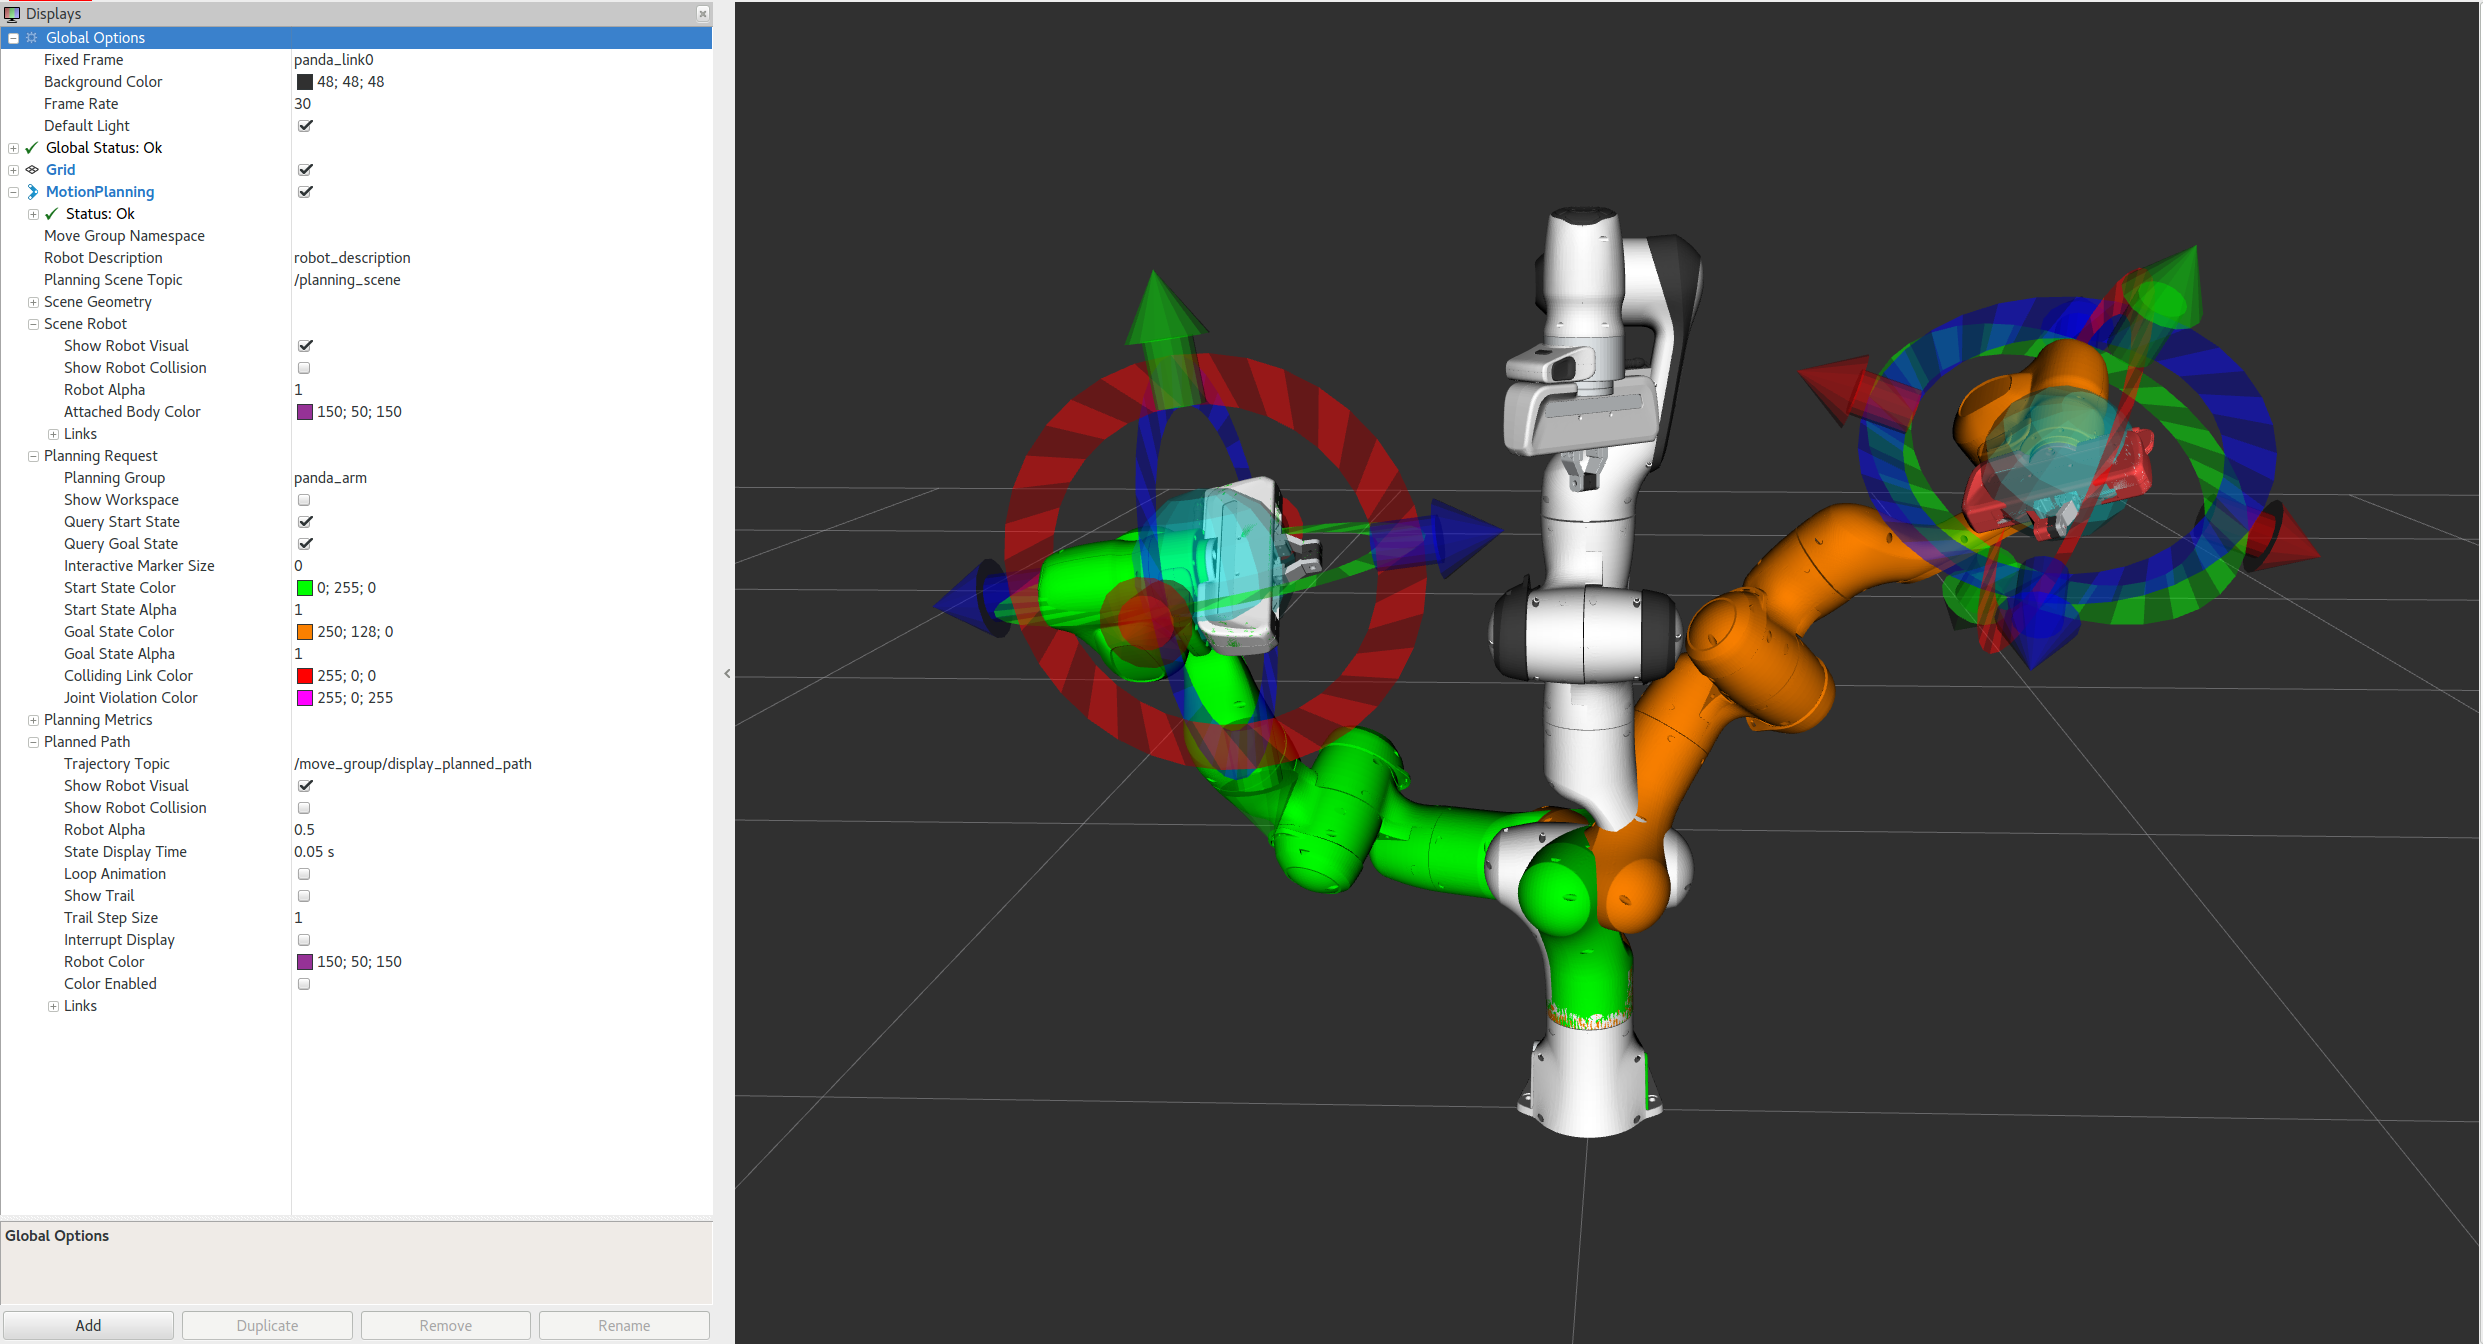
\includegraphics[width=0.8\linewidth]{moveit}
\end{center}

\end{document}



